% !TeX root = ../main.tex

% Edit this title for each week's entry.
\section{Unit 1:}
\newlecture[Introductions to PDEs][September 11, 2026]

\begin{definition}
    A PDE is an equation that relates an unkown function $u$ aNd some of its partial derivatives.
    \begin{center}
        \resizebox{\textwidth}{!}{$
            G\Big(\underbrace{x_1, \dots, x_n}_{\text{spatial coordinates}},\ \underbrace{t}_{\text{time}},\ \underbrace{u}_{\text{function}},\ \underbrace{\frac{\partial u}{\partial x_1}, \dots, \frac{\partial u}{\partial x_n}}_{\text{1st derivatives in space}},\ \underbrace{\frac{\partial u}{\partial t}}_{\text{1st derivatives in time}},\ \underbrace{\frac{\partial^2 u}{\partial x_1^2}, \frac{\partial^2 u}{\partial x_1 \partial x_2}, \dots}_{\text{2nd derivatives}}\Big) = 0
        $}
    \end{center}
\end{definition}

\begin{example}
    Model PDEs for this course.
    \\Laplace's Equation:
    \[-\Delta u = 0\]
    \[\text{Laplacian: }-\nabla \cdot \nabla = -\frac{\partial^2}{\partial x_1^2}-\frac{\partial^2}{\partial x_2^2} \text{ in }\mathbb{R}^2 \]
    Physics: potential flow, electrostatics, steady heat transfer...
\end{example}
Poisson's Equation:
\[-\Delta u = f \longleftarrow  \text{ source function: e.g. heat}\]

Heat Equation:
\[\frac{\partial u}{\partial t} - \Delta u = f \quad \text{physics: unsteady heat transfer, diffusion of chemicals...}\]
Transport Equation:
\[\frac{\partial u}{\partial t} + \underbrace{b}_{\text{advection field}} \cdot \nabla u = f \quad \text{physics: transport of conserved quantities}\]

Wave Equation:
\[\frac{\partial^2 u}{\partial t^2} - \underbrace{c^2}_{c: \text{ wave speed}} \Delta u = 0 \quad \text{physics: accousitics, vibration...}\]

Burger's Equation:
\[\frac{\partial u}{\partial t} + u\frac{\partial u}{\partial x} = 0 \quad \text{physics: nonlinear waves...}\]


\subsection{Classification of PDEs}
\begin{definition}
    The \textbf{order} of a PDE is the order of the highest derivative.
\end{definition}
\begin{example}
    \begin{align*}
        \text{Laplace's:} &\quad -\frac{\partial^2 u}{\partial x_1^2} - \frac{\partial^2 u}{\partial x_2^2} = 0 \quad \rightarrow \text{2nd order} \\
        \text{Transport:} &\quad \frac{\partial u}{\partial t} + \frac{\partial u}{\partial x} = 0 \quad \rightarrow \text{1st order} \\
        \text{Heat:} &\quad \frac{\partial u}{\partial t} - \Delta u = 0 \quad \rightarrow \text{2nd order (1st in time, 2nd in space)}
    \end{align*}
\end{example}

\begin{definition}
    An operator $\mathcal{L}$  is a \textbf{linear operator} if
    \[\mathcal{L} (\alpha w + \beta w) = \alpha \mathcal{L}  w + \beta \mathcal{L}  v\]
    for any functions $w$ \& $v$ and scalars $\alpha$ \& $\beta$
\end{definition}

\begin{definition}
    A PDE is \textbf{linear} if it can be expressed as
    \[\underbrace{\mathcal{L}}_{\text{linear operator}} u = \underbrace{f}_{\text{function independent of $u$}}\]
    If PDE is not linear, then it is a \underline{nonlinear PDE}.
\end{definition}

\begin{definition}
    A \textbf{linear homogeneous PDE} is a PDE of the form
    \[\mathcal{L} u = 0\]
    If a linear PDE is not homogeneous, then it is a \underline{linear nonhomogeneous PDE}.
\end{definition}

\begin{example}
    \begin{align*}
        \text{Laplace's:} &\quad -\Delta u =0 \quad \rightarrow \text{linear homogeneous} \\
        \text{Poisson's:} &\quad -\Delta u = f, f\neq 0 \quad \rightarrow \text{linear nonhomogeneous} \\
        \text{Heat:} &\quad \frac{\partial u}{\partial t} - \Delta u = 0 \quad \rightarrow \text{linear homogeneous}\\
        \text{Burger's:} &\frac{\partial u}{\partial t} + u \frac{\partial u}{\partial x} = 0 \quad \rightarrow \text{nonlinear}        
    \end{align*}
\end{example}

\subsection{Superposition}
\begin{itemize}
    \item If $\mathcal{L} u_1 = 0$ and $\mathcal{L} u_2 = 0$, then $\mathcal{L}(u_1+u_2)=0 $
    \item In addition, if $\mathcal{L} u_0 = f$, then $\mathcal{L}(u_0+u_1+u_2) = f$
\end{itemize}
\begin{itemize}[label = $\Rightarrow$]
    \item used frequently to solve \underline{linear} PDEs
    \item an unique solution found by imposing boundary (and initial) conditions
\end{itemize}

\subsection{Classification of Second-Order PDEs}
\begin{itemize}
    \item Consider a general linear operator of the form
    \[\mathcal{L} u = \sum_{i,j=1}^{n}a_{ij} \frac{\partial^2 u}{\partial x_i \partial y_i}+\sum_{i=1}^{n}b_i \frac{\partial u}{\partial x_i}+ cu\]
    (if problem is time-dependent, treat $t$ as 0-th coordinate)
    \item Let $A \in \mathbb{R} ^{n \times n}$ be a symmetric matrix s.t. $A_{ij} = a_{ij}$
    \item Let $\lambda_1, \dots, \lambda_n$ be the eigenvalues of $A$.
    \item Classifications:
    \begin{itemize}
        \item \textbf{elliptic}: all eigenvalues are nonzero and have same sign 
        \item \textbf{hyperbolic}: all eigenvalues are nonzero and exactly one of them have a different sibling
        \item \textbf{parabolic}: exactly one eigenvvalue is 0 and all others have the same sign
    \end{itemize}
\end{itemize}


\begin{example}

    Laplace's: $\mathcal{L} = -\Delta = -\frac{\partial^2}{\partial x_1^2} - \frac{\partial^2}{\partial x_2^2}$ in $\mathbb{R}^2$
    \[A = \begin{pmatrix} -1 & 0 \\ 0 & -1 \end{pmatrix} \quad \Rightarrow \lambda_1 = \lambda_2 = -1 \Rightarrow \text{ elliptic}\]

    Poisson's: elliptic

    Wave: $\mathcal{L} = \frac{\partial^2}{\partial t^2} - \Delta = \frac{\partial^2}{\partial t^2}- \frac{\partial^2}{\partial x_1^2} - \frac{\partial^2}{\partial x_2^2}$ (in $\mathbb{R}^2 \times \mathbb{R}$)
    \[A = \begin{pmatrix}
        1 & & \\ & -1 & \\ & & -1
    \end{pmatrix} \Rightarrow \lambda_1 = 1, \lambda_2 = \lambda_3 = -1 \Rightarrow \text{ hyperbolic}\]

    Heat: $\mathcal{L} = \frac{\partial}{\partial t} - \Delta = \frac{\partial}{\partial t} - \frac{\partial ^2}{\partial x_1^2} - \frac{\partial^2}{\partial x_2^2}$ in $\mathbb{R}^2 \times \mathbb{R} $
    \[A = \begin{pmatrix}
    0 & & \\ & -1 & \\ & & -1
    \end{pmatrix} \Rightarrow \lambda_1 = 0, \lambda_2 = \lambda_3 = -1 \Rightarrow \text{ parabolic}\]
\end{example}

\subsection{Variable Coefficient}
\[x_2 \frac{\partial ^2 u}{\partial x_1} + \frac{\partial ^2 u}{\partial x_2} = 0 \Rightarrow A = \begin{pmatrix}
    x_2 & 0 \\ 0 & 1
\end{pmatrix} \Rightarrow \lambda_1 = x_2, \lambda_2 = 1\]

\begin{center}
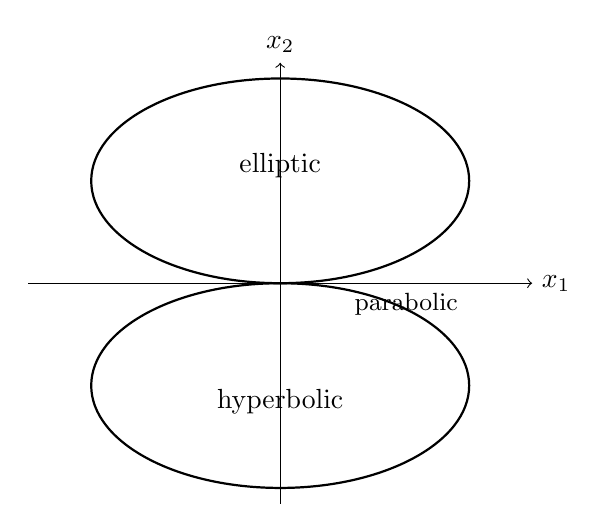
\begin{tikzpicture}[scale=1]
    \draw[->] (-3.2,0) -- (3.2,0) node[right] {$x_1$};
    \draw[->] (0,-2.8) -- (0,2.8) node[above] {$x_2$};

    \draw[thick] (0,1.3) ellipse (2.4cm and 1.3cm);
    \node at (0,1.5) {elliptic};

    \draw[thick] (0,-1.3) ellipse (2.4cm and 1.3cm);
    \node at (0,-1.5) {hyperbolic};

    \node[below] at (1.6,0) {\small parabolic};
\end{tikzpicture}
\end{center}


\newlecture[Fourier Series][September 14, 2026]
Motivation: to solve PDEs, we must represent solution $u$ as a function of space.

Given some function:
\begin{itemize}[label = ]
    \item Approach 1: describe point-wise values
    \item Approach 2: linear combination of known functions (e.g. polynomial)
    \[u(x) = \sum_{n=1}^{\infty} \hat{u}_n \varphi_n (x)\]
    $\Rightarrow$ can be easily differentiated: $u'(x) = \sum_{n=1}^{\infty}\hat{u}_n \varphi_n'(x)$
    $\Rightarrow$ classical method \underline{Fourier Series} (sin \& cos)
\end{itemize}

\begin{definition}
    $f: \mathbb{R} \rightarrow \mathbb{R} $ is \underline{$z$-periodic} if
    \[f(x+z) = f(x) \forall x \in \mathbb{R} \]
    \underline{Fundamental Period}: smallest $z$ for which the relationship holds
\end{definition}

\begin{example}
    \[f(x) = sin(x) \quad \Rightarrow \quad 2\pi \text{ periodic}\]
    \[f(x) = sin(x) + cos(2x) \quad \Rightarrow \quad 2\pi \text{ periodic}\]
\end{example}

\begin{definition}
    \(f:{ \mathbb{R} \rightarrow \mathbb{R}}\) is \underline{even} if $f(-x) = f(x)$, sym about y
    \(f: {\mathbb{R} \rightarrow \mathbb{R}}\) is \underline{odd} if $f(-x) = -f(x)$, sym about origin.
\end{definition}

\begin{definition}
    Given $f:(0, a) \rightarrow \mathbb{R}$, its \underline{periodic extension} to $\mathbb{R} $ is $f^p: \mathbb{R} \rightarrow \mathbb{R}$ such that $f^p(x) = f(x), x \in(0,a)$ and has a period of "$a$".
\end{definition}

\begin{definition}
    Given $f:(0, a) \rightarrow \mathbb{R}$, its \underline{even periodic extension} to $\mathbb{R} $ is $f^{e,p}: \mathbb{R} \rightarrow \mathbb{R}$ such that
    \[
    f^{e,p}(x) = \begin{cases}
        f(x), & x \in (0,a) \\
        f(-x), & x\in(-a, 0)
    \end{cases} \quad \text{and has a period of } 2a
    \]
\end{definition}

\begin{definition}
    Given $f:(0, a) \rightarrow \mathbb{R}$, its \underline{odd periodic extension} to $\mathbb{R} $ is $f^{o,p}: \mathbb{R} \rightarrow \mathbb{R}$ such that
    \[
    f^{o,p}(x) = \begin{cases}
        f(x), & x \in (0,a) \\
        -f(-x), & x\in(-a, 0)
    \end{cases} \quad \text{and has a period of } 2a
    \]
\end{definition}

\begin{definition}
    Let $f:\mathbb{R} \rightarrow \mathbb{R}$ be a 2-periodic function, the \rb{Fourier Series} of $f$ is
    \[f(x) ~ \frac{1}{2}a_0 + \sum_{n=1}^{\infty}(a_n cos (n\pi x) + b_n sin(n\pi x))\]
    with \underline{Fourier Coefficients}
    \[a_n = \int_{-1}^{1}cos(n \pi x)f(x)\,dx, \quad n=0,1,2,\dots\]
    \[b_ = \int_{-1}^{1}sin(n\pi x)f(x)  \,dx, \quad n = 1,2,3,\dots \]
\end{definition}

\begin{definition}
    \textbf{Truncated Fourier Series} is the partial sum
    \[S_N(x) = \frac{1}{2}a_0 + \sum_{n=1}^{N}(a_n cos(n\pi x) + b_n (n\pi x))\]
\end{definition}
Observations
\begin{enumerate}
    \item In general, the Fourier series of $f$ is \underline{not} equal to $f$, and hence we use "~" instead of "=".
    \item The set of functions
    \[\left\{\frac{1}{\sqrt{2}}, \sin(\pi x), \cos (\pi x), \sin(2\pi x), \cos(2\pi x), \dots\right\}\]
    is \underline{orthanormal} with respect to the $L^2$ inner product
    \[(w, v) = \int_{-1}^{1}wv\,dx \quad w,v,\in \mathbb{R}^2, w\cdot v = 0\]
    For all $n,m = 1,2,3\dots$
    \begin{itemize}
        \item $\int_{-1}^{1} (\frac{1}{\sqrt{2}})(cos(m \pi x))\,dx = \frac{1}{\sqrt{2}m\pi}sin(m\pi x)|^1_{x=-1} = 0$
        \item $\int_{-1}^{1} sin (m\pi x)\,dx = 0$
        \item $\int_{-1}^{1} cos(n\pi x) cos(m\pi x)\,dx - \delta_{mn} = \begin{cases}
            1 & \text{if }m=n \\
            0& \text{otherwise}
        \end{cases}$
        \item $\int_{-1}^{1} sin(n\pi x)sin(m\pi x)\,dx = \delta_{mn}$
        \item $\int_{-1}^{1} sin(n\pi x)cos(m\pi x)\,dx = 0$
    \end{itemize}
    \item Expression for Fourier coefficients are a consequence of orthogonality
    e.g. consider $a_2$
    \\ \underline{want}: $f(x) = \frac{1}{2}a_0 + \sum_{n=1}^{\infty} (a_n cos (n \pi x) + b_n sin(n\pi x))$
    \\ multiply by $cos(2\pi x)$ and integrate over $(-1,1)$
    \[\int_{-1}^{1}cos(2\pi x)f(x)  \,dx = \int_{-1}^{1}cos(2\pi x)[\frac{1}{2}a_0 + \sum_{n=1}^{\infty} (a_n cos (n\pi x) + b_n sin(n\pi x))]  \,dx  \]
    \[ = a_0 \underbrace{\int_{-1}^{1} \frac{1}{2}cos(2\pi x) \,dx }_{0} + \sum_{n=1}^{\infty} a_n \underbrace{a_n \int_{-1}^{1} cos(2\pi x)cos(n \pi x) \,dx }_{S_{n2}} + \sum_{n=1}^{\infty}\underbrace{\int_{-1}^{1} cos(2\pi x)sin(n \pi x) \,dx }_{=0}\]
    \[ = \sum_{n=1}^{\infty} a_n S_{n2} = a_2\]
    \item If $f:(-1, 1) \rightarrow \mathbb{R}$, then its Fourier series is "equal to"
    \begin{enumerate}[label = (\roman*)]
        \item $f$ as $(-1,1)$
        \item its periodic extension $f^p$ in $\mathbb{R}$
    \end{enumerate}
\end{enumerate}
\begin{example}
    \[f(x) = x \text{ for } x \in (-1,1)\]
    want: $f(x)\sim \frac{1}{2}a_0 +\sum_{n=1}^{\infty} (a_n cos(n\pi x) + b_n sin(n\pi x))$
    \[a_n = \int_{-1}^{1}f(x)cos(n\pi x)  \,dx = \int_{-1}^{1} x cos(n\pi x) \,dx =0\]
    \[b_n = \int_{-1}^{1}xsin(n\pi x)  \,dx = [\frac{sin(n\pi x)}{n^2 \pi^2}]|^1_{x=-1} - [\frac{xcos(n\pi x)}{n\pi}]|^1_{x=-1}\]
    \[-1 = -2\frac{cos(n\pi)}{n\pi}= -\frac{2(-1)^n}{n\pi} = 2\frac{(-1)^{n+1}}{n\pi}\]
    Hence, 
    \[f(x) \sim \sum_{n=1}^{\infty}b_n sin(n\pi x) = \boxed{\sum_{n=1}^{\infty} 2\frac{(-1)^{n+1}}{n\pi}sin(n\pi x)}\]
\end{example}

\begin{definition}
    Let $f: \mathbb{R} \rightarrow\mathbb{R} $ be an \underline{even $z$-periodic} function. The \rb{Fourier cosine series} is
    \[f(x) \sim \frac{1}{2}\hat{f}_0 + \sum_{n=1}^{\infty} \hat{f}_n cos(n\pi x)\]
    where $\hat{f}_n = \int_{-1}^{1} cos(n\pi x)f(x) \,dx = 2\int_{0}^{1} cos(n\pi x)f(x)  \,dx  $
    
    Let $f: \mathbb{R} \rightarrow\mathbb{R} $ be an \underline{even $z$-periodic} function. The \rb{Fourier sine series} is
    \[f(x) \sim \sum_{n=1}^{\infty} \hat{f}_n cos(n\pi x)\]
    where $\hat{f}_n = \int_{-1}^{1} sin(n\pi x)f(x) \,dx = 2\int_{0}^{1}sin(n\pi)x f(x)  \,dx $
\end{definition}
Observations:
\begin{enumerate}
    \item If $f:(0,1) \rightarrow \mathbb{R}$, then its Fourier cosine/sine series is "equal to"
    \begin{enumerate}[label = (\roman*)]
        \item $f$ as $(0,1)$ \& its even/odd periodic extension as $\mathbb{R} $
    \end{enumerate}
    \item We use $\hat{f}_n$ to denote Fourier cosine/sine coefficients of $f$
\end{enumerate}
\begin{example}
    Fourier cosine series of $f(x) = x, x \in (0,1)$
    \[\hat{f}_0 = 2\int_{0}^{1} x \,dx =1 \]
    \[\hat{f}_n = 2\int_{0}^{1}cos(n\pi x)x  \,dx = \begin{cases}
        -\frac{4}{n\pi^2}, & n \text{ odd} \\
        0, & n \text{ even}
    \end{cases} \]
    \[f(x) \sim \frac{1}{2}\hat{f}_0 + \sum_{n=1}^{\infty} \hat{f}_n cos(n \pi x) = \frac{1}{2} + \sum_{n=1, n\in \text{odd}}^{\infty}(-\frac{4}{n^2\pi^2}) cos (n\pi x)\]
    \[= \frac{1}{2} + \sum_{k=1}^{\infty} - \frac{4}{(2k-1)^2 \pi^2} cos((2k-1)\pi x)\]
\end{example}
\begin{example}
    Fourier sine series of $f(x) = x, x\in(0,1)$
    \[\hat{f}_n = 2\int_{0}^{1}sin(n\pi x)  \,dx = \cdots = \frac{2}{n\pi}(-1)^{n_1} \]
    \[f(x) \sim \sum_{n=1}^{\infty} \hat{f}_n sin(n\pi x) = \sum_{n=1}^{\infty} \frac{2(-1)^(n+1)}{n\pi}sin(n\pi x)\]
\end{example}

\b{Obstructions}:
\begin{enumerate}
    \item Coefficients follow from orthogonality
    \[\frac{1}{L} \int_{-L}^{L}\sin(\frac{n\pi x}{L})\sin(\frac{m\pi x}{L})\, dx = \delta_{mn}, \quad \text{etc}\]
    \item Given $f:(-L, L) \to \mathbb{R}$, its Fourier serires converges to $2L$ - periodic extension on $\mathbb{R}$.
\end{enumerate}